% The four slots of U, and which of them proj(U) reads.  Section 5 states
%
%     proj(U)_{i l} = sum_c U_{(i,0),(0,c)} conj(U_{(l,0),(0,c)}),
%
% and a reader meeting a four-index object for the first time cannot see from
% the formula which index is pinned, which is free and which is summed.  This
% picture says it once: warm is the allocation (the INPUT temporary is pinned
% to 0), blue are the two free OUTPUT temporary levels, plum is the visible
% index that is summed away.
%
% Drawn at d = 3, m = 2, so U is 6x6 and reads as a 3x3 array of 2x2 blocks:
% the block says which temporary levels, the cell inside it says which visible
% indices.  That is the whole point -- the block/cell split IS the (i,b),(j,c)
% split -- so the gaps between blocks are load-bearing, not decoration.
%
% WIDTH. \textwidth is 395.8pt; this is about 355pt.
%
%   make figures                               compiles it
%   \includegraphics{figures/proj-index}       includes it
\documentclass[tikz,border=3pt]{standalone}
% ---------------------------------------------------------------------------
% figures/house.tex -- the shared look. Every figure \input's this, so six
% figures look like one hand drew them instead of six.
%
% HOW FIGURES WORK HERE. tikz/pgf is NOT on ACM's production package list, so
% the documents never load it. Each figure is its own standalone document in
% this directory, compiled to a PDF by `make figures`, and pulled into a
% section with
%
%     \begin{figure}
%       \centering
%       \includegraphics{figures/my-figure}
%       \caption{What to LOOK at, not what the figure is of.}
%       \label{fig:my-figure}
%     \end{figure}
%
% Three conventions:
%   * a float sits where it is discussed;
%   * a caption says what to look at, not what the figure is of;
%   * a figure is checked by rendering it and looking, not by a clean compile.
%
% The palette below is the same as the one in preamble.tex. It is repeated
% rather than shared because these are standalone documents that never see the
% paper's preamble, so a colour changed there must be changed here too.
% ---------------------------------------------------------------------------
\usepackage{amsmath}
% The figures build with LuaLaTeX like the documents, so their text is the
% paper's Libertine and their code is the paper's Iosevka.
\usepackage{fontspec}
\setmainfont{LinLibertine_R.otf}[BoldFont=LinLibertine_RB.otf,ItalicFont=LinLibertine_RI.otf,BoldItalicFont=LinLibertine_RBI.otf,Ligatures=TeX]
\setmonofont{Iosevka Custom}[Scale=MatchLowercase,RawFeature={-liga,-calt,-clig,-dlig}]
% Math in the figures is the paper's math: acmart sets Libertinus Math under
% LuaTeX, so the letters on a wire match the letters in the text around it.
\usepackage{unicode-math}
\setmathfont{LibertinusMath-Regular.otf}
\usetikzlibrary{positioning,arrows.meta,fit,backgrounds,calc}

% Blackboard Z, which the documents get from the paper preamble.
% Kept here so a figure never reaches for the paper's preamble.
\newcommand{\Z}{\mathbb{Z}}


\definecolor{ink}{HTML}{16191D}
\definecolor{accent}{HTML}{1F4E79}
\definecolor{accentsoft}{HTML}{E8EEF4}
% accent, accentwarm and accentplum mark the temporary's basis level -- level
% 0, 1, 2 -- wherever a picture or a matrix has to show which branch is which.
\definecolor{accentwarm}{HTML}{9A5B00}
\definecolor{accentplum}{HTML}{8E2F5F}
\definecolor{muted}{HTML}{5B6470}
\definecolor{hairline}{HTML}{C9CFD6}

\tikzset{
  % Every figure inherits this: thin lines, small type, generous air.
  house/.style={
    >={Stealth[length=2.1mm, width=1.6mm]},
    line width=0.5pt,
    node distance=9mm and 15mm,
    every node/.style={font=\small},
  },
  % A thing.
  box/.style={
    draw=ink, line width=0.5pt, rounded corners=1.5pt,
    inner xsep=6pt, inner ysep=4pt, align=center,
  },
  % A thing we are drawing attention to. One per figure, at most.
  boxhi/.style={box, draw=accent, fill=accentsoft, text=ink},
  % A thing that is context, not content.
  boxdim/.style={box, draw=hairline, text=muted},
  % An arrow, and the word on it.
  flow/.style={->, draw=ink},
  flowdim/.style={->, draw=hairline},
  lbl/.style={font=\footnotesize\itshape, text=accent, inner sep=2pt},
  lbldim/.style={font=\footnotesize, text=muted, inner sep=2pt},
  % A dashed grouping rectangle behind a set of nodes.
  group/.style={draw=hairline, dashed, rounded corners=2pt, inner sep=7pt},
}


\tikzset{
  cell/.style={draw=hairline, line width=0.4pt, minimum size=6mm, inner sep=0pt,
               font=\scriptsize, text=muted},
  pick/.style={cell, draw=accent, line width=0.7pt, fill=accentsoft, text=ink},
  warmcol/.style={fill=accentwarm!8},
  ixlbl/.style={font=\scriptsize, text=muted, inner sep=1.5pt},
  ixhot/.style={font=\scriptsize, text=accent, inner sep=1.5pt},
  ixwarm/.style={font=\scriptsize, text=accentwarm, inner sep=1.5pt},
  ixplum/.style={font=\scriptsize, text=accentplum, inner sep=1.5pt},
}

\newcommand{\gap}{0.34}

\begin{document}
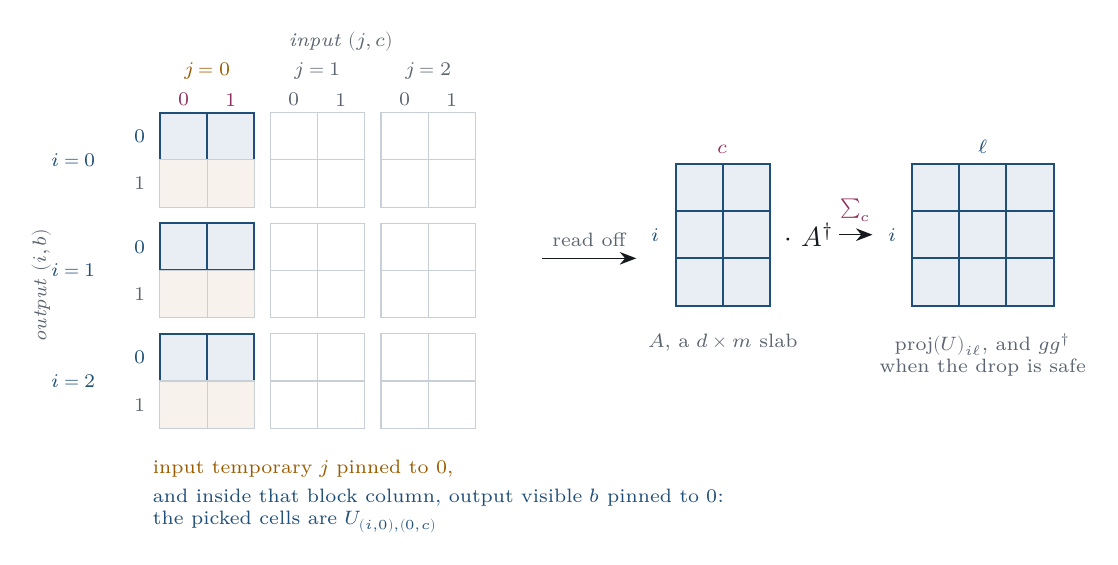
\begin{tikzpicture}[house]

% ---------------------------------------------------------------- U, 6 x 6
% cell (i,b),(j,c) sits at x = (2j+c+\gap j)*6mm, y = -(2i+b+\gap i)*6mm
\foreach \i in {0,1,2}{
  \foreach \b in {0,1}{
    \foreach \j in {0,1,2}{
      \foreach \c in {0,1}{
        \pgfmathsetmacro{\xx}{(2*\j+\c+\gap*\j)*0.6}
        \pgfmathsetmacro{\yy}{-(2*\i+\b+\gap*\i)*0.6}
        \ifnum\j=0
          \ifnum\b=0
            \node[pick] (u\i\b\j\c) at (\xx,\yy) {};
          \else
            \node[cell, warmcol] (u\i\b\j\c) at (\xx,\yy) {};
          \fi
        \else
          \node[cell] (u\i\b\j\c) at (\xx,\yy) {};
        \fi
      }}}}

% column headings: the input temporary level j (warm at j=0), then c
\foreach \j/\lab in {0/{$j=0$},1/{$j=1$},2/{$j=2$}}{
  \pgfmathsetmacro{\xm}{(2*\j+0.5+\gap*\j)*0.6}
  \ifnum\j=0
    \node[ixwarm, anchor=south] at (\xm,0.66) {\lab};
  \else
    \node[ixlbl, anchor=south] at (\xm,0.66) {\lab};
  \fi}
\foreach \j in {0,1,2}{
  \foreach \c in {0,1}{
    \pgfmathsetmacro{\xx}{(2*\j+\c+\gap*\j)*0.6}
    \ifnum\j=0
      \node[ixplum, anchor=south] at (\xx,0.32) {$\c$};
    \else
      \node[ixlbl, anchor=south] at (\xx,0.32) {$\c$};
    \fi}}
\node[ixlbl, anchor=south] at (2.0,1.02) {\textit{input} $(j,c)$};

% row headings: the output temporary level i, then b
\foreach \i in {0,1,2}{
  \pgfmathsetmacro{\ym}{-(2*\i+0.5+\gap*\i)*0.6}
  \node[ixhot, anchor=east] at (-1.05,\ym) {$i=\i$};
  \foreach \b in {0,1}{
    \pgfmathsetmacro{\yy}{-(2*\i+\b+\gap*\i)*0.6}
    \ifnum\b=0
      \node[ixhot, anchor=east] at (-0.42,\yy) {$0$};
    \else
      \node[ixlbl, anchor=east] at (-0.42,\yy) {$1$};
    \fi}}
\node[ixlbl, rotate=90, anchor=south] at (-1.62,-1.9) {\textit{output} $(i,b)$};

% what the two pinnings are: the warm column block, and the blue row of it
\node[ixwarm, anchor=north west, align=left, font=\scriptsize]
  at (-0.45,-4.05) {input temporary $j$ pinned to $0$,};
\node[ixhot, anchor=north west, align=left, font=\scriptsize]
  at (-0.45,-4.42) {and inside that block column, output visible $b$ pinned to
                    $0$:\\ the picked cells are $U_{(i,0),(0,c)}$};

% ------------------------------------------------------------------ arrow
\node[ixlbl, anchor=south] at (5.15,-1.46) {read off};
\draw[flow] (4.55,-1.55) -- (5.75,-1.55);

% ------------------------------------------------------------------- A, 3 x 2
\begin{scope}[xshift=6.55cm]
  \foreach \i in {0,1,2}{
    \foreach \c in {0,1}{
      \pgfmathsetmacro{\xx}{\c*0.6}
      \pgfmathsetmacro{\yy}{-(\i*0.6)-0.65}
      \node[pick] (a\i\c) at (\xx,\yy) {};}}
  \node[ixhot, anchor=east] at (-0.44,-1.25) {$i$};
  \node[ixplum, anchor=south] at (0.3,-0.28) {$c$};
  \node[ixlbl, anchor=north, font=\scriptsize] at (0.3,-2.45)
    {$A$, a $d \times m$ slab};
\end{scope}

% --------------------------------------------------------- A A^dagger = proj
\node[anchor=center, font=\normalsize, text=ink] at (7.95,-1.25) {$\cdot\ A^{\dagger}$};
\draw[flow] (8.32,-1.25) -- (8.75,-1.25);
\node[ixplum, anchor=south, font=\scriptsize] at (8.535,-1.15)
  {$\textstyle\sum_c$};

\begin{scope}[xshift=9.55cm]
  \foreach \i in {0,1,2}{
    \foreach \l in {0,1,2}{
      \pgfmathsetmacro{\xx}{\l*0.6}
      \pgfmathsetmacro{\yy}{-(\i*0.6)-0.65}
      \node[pick] (p\i\l) at (\xx,\yy) {};}}
  \node[ixhot, anchor=east] at (-0.44,-1.25) {$i$};
  \node[ixhot, anchor=south] at (0.6,-0.28) {$\ell$};
  \node[ixlbl, anchor=north, font=\scriptsize, align=center] at (0.6,-2.45)
    {$\mathrm{proj}(U)_{i\ell}$, and $gg^{\dagger}$\\when the drop is safe};
\end{scope}

\end{tikzpicture}
\end{document}
